\subsection*{Pochodne, monotoniczność i~ekstrema funkcji}
\subsubsection*{Zadanie~7.1.}
\begin{itemize}
    \item[g)]
        \begin{gather*}
            f\pars{x} = x^3 - 2{,}5x^2 - 2x + 1 \qquad x \in \real\\
            f'\pars{x} = 3x^2 - 5x - 2
        \end{gather*}
        Wyznaczamy miejsca zerowe pochodnej:
        \begin{gather*}
            \Delta = \pars{-5}^2 - 4 \cdot 3 \cdot \pars{-2}
                = 25 + 24
                = 49\\
            \sqrt{\Delta} = \sqrt{49} = 7\\
            x_1 = \frac{-\pars{-5} - \sqrt{\Delta}}{2 \cdot 3} = \frac{5 - 7}{6} = -\frac{1}{3}\\
            x_2 = \frac{-\pars{-5} + \sqrt{\Delta}}{2 \cdot 3} = \frac{5 + 7}{6} = 2\\
            \upparabola{-\frac{1}{3}}{2}\\
            \tag{\(1\)} \forall x \in \open{-\infty}{0}\colon f'\pars{x} > 0 \label{2020_10_20:7_1:g:first_increase}\\
            \tag{\(2\)} f'\pars{-\frac{1}{3}} = 0 \label{2020_10_20:7_1:g:first_zero}\\
            \tag{\(3\)} \forall x \in \open{-\frac{1}{3}}{2}\colon f'\pars{x} < 0 \label{2020_10_20:7_1:g:decrease}\\
            \tag{\(4\)} f'\pars{2} = 0 \label{2020_10_20:7_1:g:second_zero}\\
            \tag{\(5\)} \forall x \in \open{2}{+\infty}\colon f'\pars{x} > 0 \label{2020_10_20:7_1:g:second_increase}\\
        \end{gather*}
        Co z~tego wynika:
        \begin{description}
            \item \(\mbox{(\ref{2020_10_20:7_1:g:first_increase})} \implies\) funkcja \(f\) jest rosnąca w~przedziale \(\open{-\infty}{-\frac{1}{3}}\)
            \item \(\mbox{(\ref{2020_10_20:7_1:g:first_increase})} \land \mbox{(\ref{2020_10_20:7_1:g:first_zero})} \land \mbox{(\ref{2020_10_20:7_1:g:decrease})} \implies\) funkcja \(f\) ma maksimum lokalne w~punkcie \(x = -\frac{1}{3}\):
                \begin{equation*}
                    f\pars{-\frac{1}{3}}
                        = -\frac{1}{27} - \frac{5}{2} \cdot \frac{1}{9} + \frac{2}{3} + 1
                        = -\frac{2}{54} - \frac{15}{54} + \frac{36}{54} + 1
                        = \frac{73}{54}
                \end{equation*}
            \item \(\mbox{(\ref{2020_10_20:7_1:g:decrease})} \implies\) funkcja \(f\) jest malejąca w~przedziale \(\open{-\frac{1}{3}}{2}\)
            \item \(\mbox{(\ref{2020_10_20:7_1:g:decrease})} \land \mbox{(\ref{2020_10_20:7_1:g:second_zero})} \land \mbox{(\ref{2020_10_20:7_1:g:second_increase})} \implies\) funkcja \(f\) ma minimum lokalne w~punkcie \(x = 2\):
                \begin{equation*}
                    f\pars{2}
                        = 2^3 - \frac{5}{2} \cdot 4 - 4 + 1
                        = 8 - 10 - 4 + 1
                        = -5
                \end{equation*}
            \item \(\mbox{(\ref{2020_10_20:7_1:g:second_increase})} \implies\) funkcja \(f\) jest rosnąca w~przedziale \(\open{2}{+\infty}\)
        \end{description}
\end{itemize}
\subsubsection*{Zadanie~7.2.}
\begin{itemize}
    \item[g)]
        \begin{gather*}
            f\pars{x} = \frac{1}{4}x^4 - \frac{5}{3}x^3 + 3x^2 + 2 \qquad x \in \real\\
            f'\pars{x} = x^3 - 5x^2 + 6x = x\pars{x^2 - 5x + 6} = x\pars{x - 2}\pars{x - 3}\\
            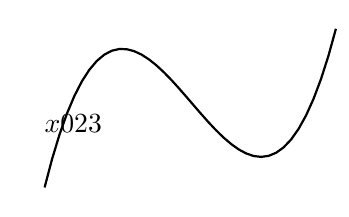
\begin{tikzpicture}
                \drawvec (-1, 0) -- (4, 0) node[below]{\(x\)};
                \draw[thick, samples=40, domain=-0.2:3.5] plot (\x, {0.5 * \x * (\x - 2) * (\x - 3)});
                \fillpoint*{0, 0}[\(0\)][below right];
                \fillpoint*{2, 0}[\(2\)][below left];
                \fillpoint*{3, 0}[\(3\)][below right];
            \end{tikzpicture}\\
            \tag{\(1\)} \forall x \in \open{-\infty}{0}\colon f'\pars{x} < 0 \label{2020_10_20:7_2:g:first_decrease}\\
            \tag{\(2\)} f'\pars{0} = 0 \label{2020_10_20:7_2:g:first_zero}\\
            \tag{\(3\)} \forall x \in \open{0}{2}\colon f'\pars{x} > 0 \label{2020_10_20:7_2:g:first_increase}\\
            \tag{\(4\)} f'\pars{2} = 0 \label{2020_10_20:7_2:g:second_zero}\\
            \tag{\(5\)} \forall x \in \open{2}{3}\colon f'\pars{x} < 0 \label{2020_10_20:7_2:g:second_decrease}\\
            \tag{\(6\)} f'\pars{3} = 0 \label{2020_10_20:7_2:g:third_zero}\\
            \tag{\(7\)} \forall x \in \open{3}{+\infty}\colon f'\pars{x} > 0 \label{2020_10_20:7_2:g:second_increase}\\
        \end{gather*}
        Co z~tego wynika:
        \begin{description}
            \item \(\mbox{(\ref{2020_10_20:7_2:g:first_decrease})} \implies\) funkcja \(f\) jest malejąca w~przedziale \(\open{-\infty}{0}\)
            \item \(\mbox{(\ref{2020_10_20:7_2:g:first_decrease})} \land \mbox{(\ref{2020_10_20:7_2:g:first_zero})} \land \mbox{(\ref{2020_10_20:7_2:g:first_increase})} \implies\) funkcja \(f\) ma minimum lokalne w~punkcie \(x = 0\):
                \begin{equation*}
                    f\pars{0} = 2
                \end{equation*}
            \item \(\mbox{(\ref{2020_10_20:7_2:g:first_increase})} \implies\) funkcja \(f\) jest rosnąca w~przedziale \(\open{0}{2}\)
            \item \(\mbox{(\ref{2020_10_20:7_2:g:first_increase})} \land \mbox{(\ref{2020_10_20:7_2:g:second_zero})} \land \mbox{(\ref{2020_10_20:7_2:g:second_decrease})} \implies\) funkcja \(f\) ma maksimum lokalne w~punkcie \(x = 2\):
                \begin{equation*}
                    f\pars{2} = \frac{1}{4} \cdot 2^4 - \frac{5}{3} \cdot 2^3 + 3 \cdot 2^2 + 2 = 4 - \frac{40}{3} + 12 + 2 = \frac{14}{3}
                \end{equation*}
            \item \(\mbox{(\ref{2020_10_20:7_2:g:second_decrease})} \implies\) funkcja \(f\) jest malejąca w~przedziale \(\open{2}{3}\)
            \item \(\mbox{(\ref{2020_10_20:7_2:g:second_decrease})} \land \mbox{(\ref{2020_10_20:7_2:g:third_zero})} \land \mbox{(\ref{2020_10_20:7_2:g:second_increase})} \implies\) funkcja \(f\) ma minimum lokalne w~punkcie \(x = 3\):
                \begin{equation*}
                    f\pars{3} = \frac{1}{4} \cdot 3^4 - \frac{5}{3} \cdot 3^3 + 3 \cdot 3^2 + 2 = \frac{81}{4} - 45 + 27 + 2 = \frac{17}{4}
                \end{equation*}
            \item \(\mbox{(\ref{2020_10_20:7_2:g:second_increase})} \implies\) funkcja \(f\) jest rosnąca w~przedziale \(\open{3}{+\infty}\)
        \end{description}
\end{itemize}
\subsubsection*{Zadanie~7.3.}
\begin{itemize}
    \item[g)]
        \begin{gather*}
            f\pars{x} = \frac{x^2 - 2x + 3}{x^2 + 2x - 3} = \frac{x^2 - 2x + 3}{\pars{x + 3}\pars{x - 1}} \qquad x \in \open{-\infty}{-3} \cup \open{-3}{1} \cup \open{1}{+\infty}\\
            \begin{split}
                f'\pars{x}
                    &= \frac{\pars{x^2 - 2x + 3}'\pars{x^2 + 2x - 3} - \pars{x^2 - 2x + 3}\pars{x^2 + 2x - 3}'}{\pars{x + 3}^2\pars{x - 1}^2}\\
                    &= \frac{\pars{2x - 2}\pars{x^2 + 2x - 3} - \pars{x^2 - 2x + 3}\pars{2x + 2}}{\pars{x + 3}^2\pars{x - 1}^2}\\
                    &= \frac{2x^3 + 4x^2 - 6x - 2x^2 - 4x + 6 - 2x^3 - 2x^2 + 4x^2 + 4x - 6x - 6}{\pars{x + 3}^2\pars{x - 1}^2}\\
                    &= \frac{4x^2 - 12x}{\pars{x + 3}^2\pars{x - 1}^2}
                    = \frac{4x\pars{x - 3}}{\pars{x + 3}^2\pars{x - 1}^2}
            \end{split}
        \end{gather*}
        Ponieważ wyrażenie \(\pars{x + 3}^2\pars{x - 1}^2\) jest zawsze nieujemne, to aby zbadać znak pochodnej wystarczy zbadać znak wyrażenia
        \begin{equation*}
            \frac{4x}{x - 3}
        \end{equation*}
        co z~kolei sprowadza się do zbadania znaku wyrażenia
        \begin{gather*}
            4x\pars{x - 3}\\
            \upparabola{0}{3}\\
            \tag{\(1\)} \forall x \in \open{-\infty}{-3} \cup \open{-3}{0}\colon f'\pars{x} > 0 \label{2020_10_20:7_3:g:first_increase}\\
            \tag{\(2\)} f'\pars{0} = 0 \label{2020_10_20:7_3:g:first_zero}\\
            \tag{\(3\)} \forall x \in \open{0}{1} \cup \open{1}{3}\colon f'\pars{x} < 0 \label{2020_10_20:7_3:g:decrease}\\
            \tag{\(4\)} f'\pars{3} = 0 \label{2020_10_20:7_3:g:second_zero}\\
            \tag{\(5\)} \forall x \in \open{3}{+\infty}\colon f'\pars{x} > 0 \label{2020_10_20:7_3:g:second_increase}
        \end{gather*}
        Co z~tego wynika:
        \begin{description}
            \item \(\mbox{(\ref{2020_10_20:7_3:g:first_increase})} \implies\) funkcja \(f\) jest rosnąca w~przedziałach \(\open{-\infty}{-3}\) i~\(\open{-3}{0}\)
            \item \(\mbox{(\ref{2020_10_20:7_3:g:first_increase})} \land \mbox{(\ref{2020_10_20:7_3:g:first_zero})} \land \mbox{(\ref{2020_10_20:7_3:g:decrease})} \implies\) funkcja \(f\) ma minimum lokalne w~punkcie \(x = 0\):
                \begin{equation*}
                    f\pars{0} = \frac{3}{-3} = -1
                \end{equation*}
            \item \(\mbox{(\ref{2020_10_20:7_3:g:decrease})} \implies\) funkcja \(f\) jest malejąca w~przedziałach \(\open{0}{1}\) i~\(\open{1}{3}\)
            \item \(\mbox{(\ref{2020_10_20:7_3:g:decrease})} \land \mbox{(\ref{2020_10_20:7_3:g:second_zero})} \land \mbox{(\ref{2020_10_20:7_3:g:second_increase})} \implies\) funkcja \(f\) ma minimum lokalne w~punkcie \(x = 3\):
                \begin{equation*}
                    f\pars{3} = \frac{3^2 - 2 \cdot 3 + 3}{3^2 + 2 \cdot 3 - 3} = \frac{9 - 6 + 3}{9 + 6 - 3} = \frac{6}{12} = \frac{1}{2}
                \end{equation*}
            \item \(\mbox{(\ref{2020_10_20:7_3:g:second_increase})} \implies\) funkcja \(f\) jest rosnąca w~przedziale \(\open{3}{+\infty}\)
        \end{description}
    \item[j)]
        \begin{gather*}
            f\pars{x} = x\sqrt{2x + 3}\qquad x \in \leftclosed{-\frac{3}{2}}{+\infty}\\
            f'\pars{x}
                = \pars{x\sqrt{2x + 3}}'
                = x \cdot \frac{1}{2\sqrt{2x + 3}} \cdot 2 + \sqrt{2x + 3}
                = \frac{x + 2x + 3}{\sqrt{2x + 3}}
                = \frac{3x + 3}{\sqrt{2x + 3}} \qquad x \in \open{-\frac{2}{3}}{+\infty}
        \end{gather*}
        Ponieważ wyrażenie w~mianowniku jest zawsze dodatnie, do zbadania znaku pochodnej wystarczy zbadać znak licznika. Licznik jest natomiast funkcją liniową o~miejscu zerowym \(x_0 = -1\):
        \begin{gather*}
            \begin{tikzpicture}
                \drawvec (-2, 0) -- (2, 0) node[below]{\(x\)};
                \draw[thick] (-2, -1) -- (1, 2);
                \fillpoint*{-1, 0}[\(-1\)][below right];
            \end{tikzpicture}\\
            \tag{\(1\)} \forall x \in \open{-\infty}{-1}\colon f'\pars{x} < 0 \label{2020_10_20:7_3:j:decrease}\\
            \tag{\(2\)} f'\pars{-1} = 0 \label{2020_10_20:7_3:j:zero}\\
            \tag{\(3\)} \forall x \in \open{-1}{+\infty}\colon f'\pars{x} > 0 \label{2020_10_20:7_3:j:increase}\\
        \end{gather*}
        Co z~tego wynika:
        \begin{description}
            \item \(\mbox{(\ref{2020_10_20:7_3:j:decrease})} \implies\) funkcja \(f\) jest malejąca w~przedziale \(\open{-\infty}{-1}\)
            \item \(\mbox{(\ref{2020_10_20:7_3:j:decrease})} \land \mbox{(\ref{2020_10_20:7_3:j:zero})} \land \mbox{(\ref{2020_10_20:7_3:j:increase})} \implies\) funkcja \(f\) ma minimum lokalne w~punkcie \(x = -1\):
                \begin{equation*}
                    f\pars{-1} = -1 \cdot \sqrt{2 \cdot -1 + 3} = -1
                \end{equation*}
            \item \(\mbox{(\ref{2020_10_20:7_3:j:increase})} \implies\) funkcja \(f\) jest rosnąca w~przedziale \(\open{-1}{+\infty}\)
        \end{description}
\end{itemize}
\subsubsection*{Zadanie~7.5.}
\begin{itemize}
    \item[a)]
        \begin{gather*}
            f\pars{x} = \sqrt{3}\sin x - \cos x\\
            \begin{split}
                f'\pars{x}
                    &= \sin x + \sqrt{3}\cos x
                    = \sqrt{1^2 + \pars{\sqrt{3}}^2}\pars{\frac{1}{\sqrt{1^2 + \pars{\sqrt{3}}^2}}\cdot \sin x + \frac{\sqrt{3}}{\sqrt{1^2 + \pars{\sqrt{3}}^2}} \cdot \cos x}\\
                    &= 2\pars{\frac{1}{2}\sin x + \frac{\sqrt{3}}{2}\cos x} = 2\pars{\cos\frac{\pi}{3}\sin x + \sin\frac{\pi}{3}\cos x}
                    = 2\sin\pars{x + \frac{\pi}{3}}
            \end{split}\\
            \tag{\(1\)} \forall k \in \integer\colon \forall x \in \open{2k\pi - \frac{\pi}{3}}{2k\pi + \frac{2\pi}{3}}\colon f'\pars{x} > 0 \label{2020_10_20:7_5:a:increase}\\
            \tag{\(2\)} \forall k \in \integer\colon f'\pars{2k\pi + \frac{2\pi}{3}} = 0 \label{2020_10_20:7_5:a:first_zero}\\
            \tag{\(3\)} \forall k \in \integer\colon \forall x \in \open{2k\pi + \frac{2\pi}{3}}{2k\pi + \frac{5\pi}{3}}\colon f'\pars{x} < 0 \label{2020_10_20:7_5:a:decrease}\\
            \tag{\(4\)} \forall k \in \integer\colon f'\pars{2k\pi + \frac{5\pi}{3}} = 0 \label{2020_10_20:7_5:a:second_zero}
        \end{gather*}
        Co z~tego wynika:
        \begin{description}
            \item \(\mbox{(\ref{2020_10_20:7_5:a:increase})} \implies \forall k \in \integer\colon\) funkcja \(f\) jest rosnąca w~przedziale \(\open{2k\pi - \frac{\pi}{3}}{2k\pi + \frac{2\pi}{3}}\)
            \item \(\mbox{(\ref{2020_10_20:7_5:a:increase})} \land \mbox{(\ref{2020_10_20:7_5:a:first_zero})} \land \mbox{(\ref{2020_10_20:7_5:a:decrease})} \implies \forall k \in \integer\colon\) funkcja \(f\) ma w~punkcie \(x = 2k\pi + \frac{2\pi}{3}\) lokalne maksimum:
                \begin{equation*}
                    f\pars{2k\pi + \frac{2\pi}{3}}
                        = \sqrt{3}\sin\pars{2k\pi + \frac{2\pi}{3}} - \cos\pars{2k\pi + \frac{2\pi}{3}}
                        = \sqrt{3}\sin\frac{\pi}{3} - \pars{-\sin\frac{\pi}{6}}
                        = \frac{3}{2} + \frac{1}{2}
                        = 2
                \end{equation*}
            \item \(\mbox{(\ref{2020_10_20:7_5:a:decrease})} \implies \forall k \in \integer\colon\) funkcja \(f\) jest malejąca w~przedziale \(\open{2k\pi + \frac{2\pi}{3}}{2k\pi + \frac{5\pi}{3}}\)
            \item \(\mbox{(\ref{2020_10_20:7_5:a:decrease})} \land \mbox{(\ref{2020_10_20:7_5:a:second_zero})} \land \mbox{(\ref{2020_10_20:7_5:a:increase})} \implies \forall k \in \integer\colon\) funkcja \(f\) ma w~punkcie \(x = 2k\pi + \frac{5\pi}{3}\) lokalne minimum:
                \begin{equation*}
                    f\pars{2k\pi + \frac{5\pi}{3}}
                        = \sqrt{3}\sin\pars{2k\pi + \frac{5\pi}{3}} - \cos\pars{2k\pi + \frac{5\pi}{3}}
                        = -\sqrt{3}\sin\frac{\pi}{3} - \sin\frac{\pi}{6}
                        = \frac{3}{2} - \frac{1}{2}
                        = -2
                \end{equation*}
        \end{description}
    \item[f)]
        \begin{gather*}
            f\pars{x} = \cos x + \frac{\sqrt{3}}{2}x \qquad x \in \real\\
            f'\pars{x} = -\sin x + \frac{\sqrt{3}}{2}
        \end{gather*}
        Aby zbadać znak pochodnej, rozwiążmy najpierw równanie:
        \begin{gather*}
            f'\pars{x} = 0\\
            -\sin x + \frac{\sqrt{3}}{2} = 0\\
            \sin x = \frac{\sqrt{3}}{2}\\
            x = 2k\pi + \frac{\pi}{3} \wlor x = 2k\pi + \frac{2\pi}{3}
        \end{gather*}
        Teraz na podstawie szkicu wykresu możemy zbadać, kiedy pochodna jest dodatnia:
        \begin{gather*}
            -\sin x + \frac{\sqrt{3}}{2} > 0\\
            \sin x < \frac{\sqrt{3}}{2}
        \end{gather*}
        \begin{mathfigure*}
            \def\value{\fpeval{sqrt(3) / 2}}
            \drawcoordsystem{-2.5 * pi, -1.5}{2.5 * pi, 1.5};
            \draw[thick, samples=60, domain=-2.5*pi:2.5*pi, ForestGreen, smooth] plot (\x, {sin(\x r)});
            \draw[domain=-2.5*pi:2.5*pi, thick, RoyalBlue] plot (\x, {\value});
            \drawpoint*{pi/3, \value}[\(\frac{\pi}{3}\)][above];
            \drawpoint*{2*pi/3, \value}[\(\frac{2\pi}{3}\)][above];
            \drawpoint*{7*pi/3, \value}[\(\frac{7\pi}{3}\)][above];
            \drawpoint*{-4*pi/3, \value}[\(-\frac{4\pi}{3}\)][above];
            \drawpoint*{-5*pi/3, \value}[\(-\frac{5\pi}{3}\)][above];
        \end{mathfigure*}
        Zatem
        \begin{gather*}
            \tag{\(1\)} \forall k \in \integer\colon \forall x \in \open{2k\pi - \frac{4\pi}{3}}{2k\pi + \frac{\pi}{3}}\colon f'\pars{x} > 0 \label{2020_10_20:7_5:f:increase}\\
            \tag{\(2\)} \forall k \in \integer\colon f'\pars{2k\pi + \frac{\pi}{3}} = 0 \label{2020_10_20:7_5:f:first_zero}\\
            \tag{\(3\)} \forall k \in \integer\colon \forall x \in \open{2k\pi + \frac{\pi}{3}}{2k\pi + \frac{2\pi}{3}}\colon f'\pars{x} < 0 \label{2020_10_20:7_5:f:decrease}\\
            \tag{\(4\)} \forall k \in \integer\colon f'\pars{2k\pi + \frac{2\pi}{3}} = 0 \label{2020_10_20:7_5:f:second_zero}
        \end{gather*}
        Co z~tego wynika:
        \begin{description}
            \item \(\mbox{(\ref{2020_10_20:7_5:f:increase})} \implies \forall k \in \integer\colon\) funkcja \(f\) jest rosnąca w~przedziale \(\open{2k\pi - \frac{4\pi}{3}}{2k\pi + \frac{\pi}{3}}\)
            \item \(\mbox{(\ref{2020_10_20:7_5:f:increase})} \land \mbox{(\ref{2020_10_20:7_5:f:first_zero})} \land \mbox{(\ref{2020_10_20:7_5:f:decrease})} \implies \forall k \in \integer\colon\) funkcja \(f\) ma w~punkcie \(x = 2k\pi + \frac{\pi}{3}\) maksimum lokalne:
                \begin{equation*}
                    f\pars{2k\pi + \frac{\pi}{3}}
                        = \cos\pars{2k\pi + \frac{\pi}{3}} + \frac{\sqrt{3}}{2} \cdot \pars{2k\pi + \frac{\pi}{3}}
                        = \frac{1}{2} + \frac{\sqrt{3}}{2} \cdot \pars{2k\pi + \frac{\pi}{3}}
                \end{equation*}
            \item \(\mbox{(\ref{2020_10_20:7_5:f:decrease})} \implies \forall k \in \integer\colon\) funkcja \(f\) jest malejąca w~przedziale \(\open{2k\pi + \frac{\pi}{3}}{2k\pi + \frac{2\pi}{3}}\)
            \item \(\mbox{(\ref{2020_10_20:7_5:f:decrease})} \land \mbox{(\ref{2020_10_20:7_5:f:second_zero})} \land \mbox{(\ref{2020_10_20:7_5:f:increase})} \implies \forall k \in \integer\colon\) funkcja \(f\) ma w~punkcie \(x = 2k\pi + \frac{2\pi}{3}\) minimum lokalne:
                \begin{equation*}
                    f\pars{2k\pi + \frac{2\pi}{3}}
                        = \cos\pars{2k\pi + \frac{2\pi}{3}} + \frac{\sqrt{3}}{2} \cdot \pars{2k\pi + \frac{2\pi}{3}}
                        = -\frac{1}{2} + \frac{\sqrt{3}}{2} \cdot \pars{2k\pi + \frac{2\pi}{3}}
                \end{equation*}
        \end{description}
\end{itemize}
\subsubsection*{Zadanie~7.6.}
\begin{itemize}
    \item[a)]
        \begin{gather*}
            f\pars{x} = \frac{a^2 - 1}{3}x^3 + \pars{a - 1}x^2 + 2x + 5 \qquad x \in \real\\
            f'\pars{x} = \pars{a^2 - 1}x^2 + 2\pars{a - 1}x + 2
        \end{gather*}
        Aby funkcja była rosnąca w~\(\real\), jej pochodna musi być zawsze dodatnia. Rozważmy najpierw dwa przypadki:
        \begin{proofcases}
            \item \(a = 1\)
                \begin{equation*}
                    f'\pars{x} = 2
                \end{equation*}
                Zatem \(a = 1\) jest jedną z~pasujących wartości parametru \(a\).
            \item \(a = -1\)
                \begin{equation*}
                    f\pars{x} -4x + 2
                \end{equation*}
                Taka funkcja jest ujemna, np. dla argumentu \(-1\), zatem nie spełnia warunków.
        \end{proofcases}
        Załóżmy teraz, że \(a^2 - 1 \neq 0\). Mamy zatem funkcję kwadratową. Chcemy, aby była ona zawsze dodatnia, czyli aby współczynnik przy \(x^2\) był dodatni i~aby \(\Delta\) była ujemna. Zatem:
        \begin{gather*}
            a^2 - 1 > 0\\
            a^2 > 1\\
            a \in \open{-\infty}{-1} \cup \open{1}{+\infty}\\
            \Delta < 0\\
            \pars{2\pars{a - 1}}^2 - 4 \cdot \pars{a^2 - 1} \cdot 2 < 0\\
            4a^2 - 8a + 4 - 8a^2 + 8 < 0\\
            4a^2 + 8a - 12 > 0\\
            a^2 + 2a - 3 > 0\\
            \pars{a + 3}\pars{a - 1} > 0\\
            \upparabola{-3}{1}\\
            a \in \open{-\infty}{-3} \cup \open{1}{+\infty}
        \end{gather*}
        Zatem ostatecznie \(a \in \open{-\infty}{-3} \cup \leftclosed{1}{+\infty}\).
\end{itemize}
\subsubsection*{Zadanie~7.8.}
\begin{gather*}
    f\pars{x} = \cos x - px \qquad x \in \real\\
    f'\pars{x} = -\sin x - p
\end{gather*}
Aby funkcja \(f\) była malejąca w~zbiorze \(\real\), to jej pochodna musi być zawsze ujemna. Funkcja \(-\sin x\) jest ograniczona następująco:
\begin{equation*}
    -1 \leq -\sin x \leq 1
\end{equation*}
Zatem \(-p < -1\), czyli \(p > 1\).

